% !TeX spellcheck = en_US
\section{Quantifying the delay to recover normal levels of decline due to a drop in the vaccination coverage}\label{Resilence}
In Denmark, the vaccination program started in $2009$ with a coverage of $80\%$. After $5$ years, in $2$ months the coverage dropped until $10\%$. It remained $2$ years in $10\%$ and then, in $5$ years increased until $70\%$ and remained constant. In Figure \ref{fig:cobertura_danesa} we show the coverage evolution. 

\begin{figure}[h!]
	\centering
	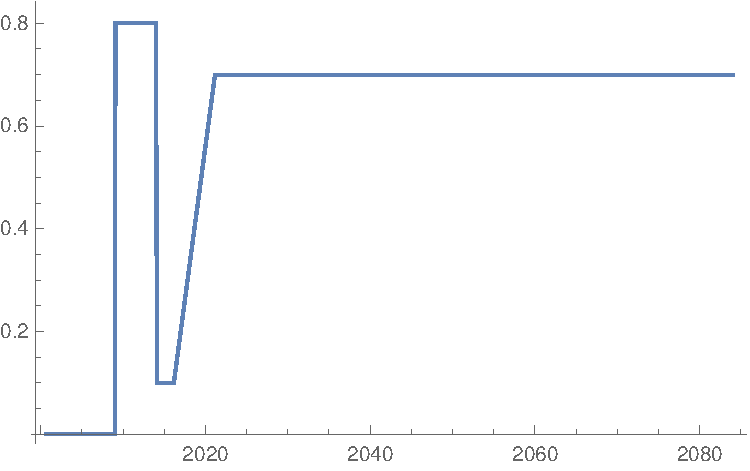
\includegraphics[width=0.5\linewidth]{IMGs/11.-Resilencia/Cobertura_Danesa.pdf}
	\caption{Evolution of the HPV vaccine coverage in Denmark from the program starting in 2009.}
	\label{fig:cobertura_danesa}
\end{figure}

Drops in the coverage have happened in some countries and it is a concerning issue because the natural consequence is the delay in achieving high rates of protection (resilience) in order to reduce the pathologies associated to HPV.

Thus, here, we are going to perform simulations to study the delay produced due to a drop in the coverage under different circumstances. A first approach has published in \cite{Elfstrm2015}, where the authors consider an age-structured model of differential equations \cite{Baussano2013} to simulate the following vaccination programs

\begin{enumerate}
	\item Case 1 or base case: vaccination of $80.5\%$ girls aged 11-12 and $53.25\%$ of the girls aged 13-18.
	\item Case 2: base case $+$ vaccination of $80.50\%$ of women aged 22-26 during the year 2015.
	\item Case 3: Case 2 $+$ vaccination of $80.50\%$ of the boys aged 11-12.
	\item Case 4: Case 3 $+$ vaccination of $80.50\%$ of the boys aged 13-26 during the year 2015.
\end{enumerate}

The above strategies are consistent with the Swedish policies, where they started vaccinating girls since 2007. The authors assume a vaccination effectiveness of $95\%$ in the vaccination of 11-12 years old boys and girls and $92\%$ for older ones.

The results obtained in \cite{Elfstrm2015} say that the vaccination programs are more resilent when only girls are vaccinated, that is, the effect of a drop in the coverage is greater if only girls are vaccinated because the decline in HPV infection is recovered faster if boys and girls are vaccinated. Also, they say that \textit{if vaccination coverage is high, $25-30$ years after vaccination commences, the effectiveness converges. The most salient impact of male vaccination is the mitigation of loss of vaccine effectiveness in the face of an unexpected reduction in coverage}.

Our goal here is to see if using our model and scenarios adapted to the Spanish situation, we are able to obtain similar results to the those in \cite{Elfstrm2015}. In our case, we propose the following scenarios

\begin{enumerate}
	\item Case 1 or base case: vaccination of $14$ years old girls with a coverage of $70\%$ starting in Oct $2007$ (current situation in Spain).
	\item Case 2: base case $+$ vaccination of $14$ years old boys with a coverage of $70\%$ starting in January $2020$.
	\item Case 3: base case $+$ in January $2025$, in $2$ months the coverage drops until $10\%$, it remains $2$ years in $10\%$ and then, in $5$ years increases until $70\%$ and remains constant (Danish scenario).
	\item Case 4: Case 2 $+$ Danish scenario starting in January 2025 droping the coverage in boys and girls (Danish scenario for both boys and girls).
\end{enumerate}

Here, we assume an effectiveness of $96.5\%$ and the use of GARDASIL9. We do not have scenarios with catchup vaccination, because in \cite{Skufca}, as we mentioned previously, the authors perform a literature review where they show that the effectiveness of the HPV vaccine on cervical abnormalities is between $20\% - 54\%$ instead of the assumed $96.5\%$ or $92\%$ assumed in \cite{Elfstrm2015}. 

%Recall that we performed a simulation with the data appearing in \cite{Skufca} in Section \ref{sec:australia_sfuka} in page \pageref{sec:australia_sfuka} and we concluded that the catch-up effectiveness for genital warts may be higher than the figures collected in \cite{Skufca} but far from $92\%$. Thus, it seems to be clear that the vaccine effectiveness experiments a reduction in those women who had previous contact with the virus.

In order to study the resilience, we are going to compare the delay produced in the decline of infections between, on the one hand, the Base Case and the Case 3 (only girls vaccination), and on the other hand, the Case 1 and the Case 4 (vaccination of boys and girls). 

We show the obtained results in Figures \ref{fig:baseCase_Case3} and \ref{fig:Case2_Case4}. Figure \ref{fig:baseCase_Case3} depicts the comparison between the Base Case and the Case 3 and Figure \ref{fig:Case2_Case4} the comparison between the Case 2 and the Case 4. In both figures, on the left column we can see the evolution over the time of the decline of the oncogenic HPV in men, women and MSM (only in Figure \ref{fig:Case2_Case4}), from year $2025$ (when the drop starts). On the right column, we visualize the average number of years the simulation with the drop in the coverage needs to achieve the same level of decline as the simulation without drop, from year $2025$ until $2055$. The difference of years to achieve the same decline is calculated as follows: for each time instant, we find the average decline level in the case where there is not drop. Then, we seek in which time instant the same average decline level is reached in the case there is drop and we calculate the difference between both time instants and divided by $12$.

In Figure \ref{fig:baseCase_Case3}, MSM are not considered because there is not herd immunity effect nor decline on them when only girls are vaccinated.  

\begin{figure}[!]
	\centering
	\begin{tabular}{cc}
		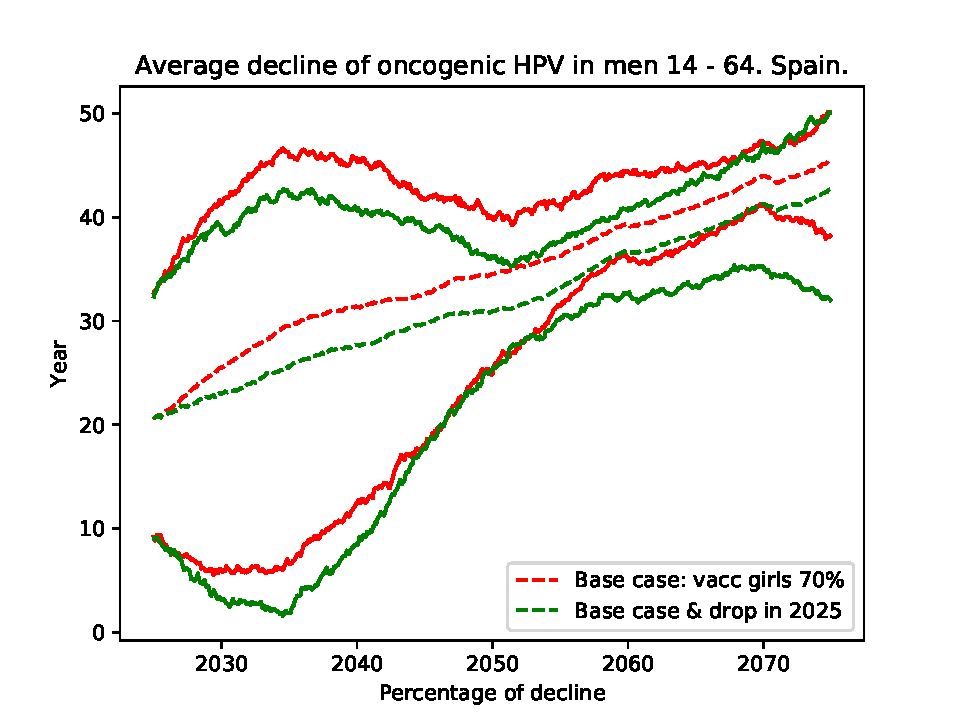
\includegraphics[width=0.5\linewidth]{IMGs/11.-Resilencia/Base_y_3/decline_onco_hom.pdf}	& 
		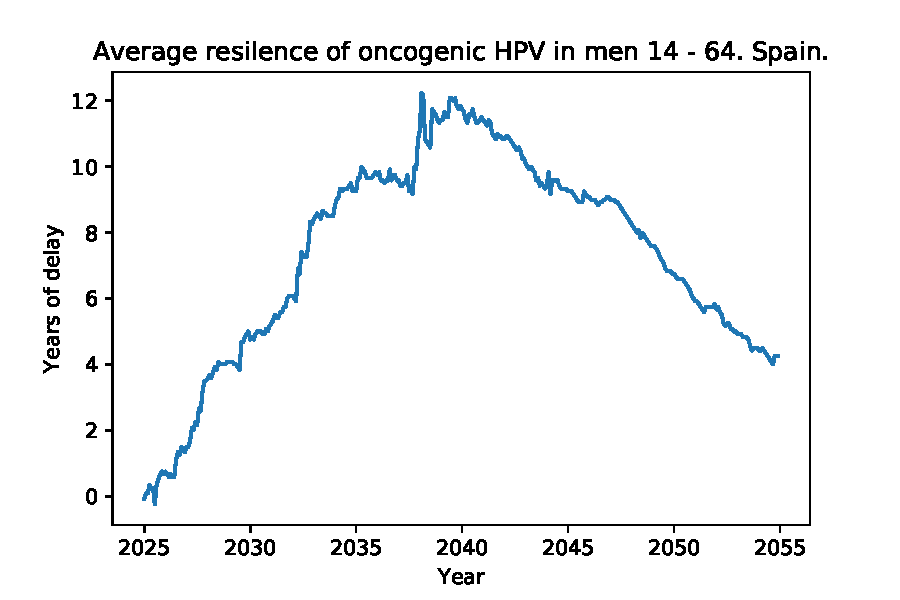
\includegraphics[width=0.5\linewidth]{IMGs/11.-Resilencia/Base_y_3/resilencia_onco_hom.pdf}  \\ 
		(a)	& (b) \\ 
		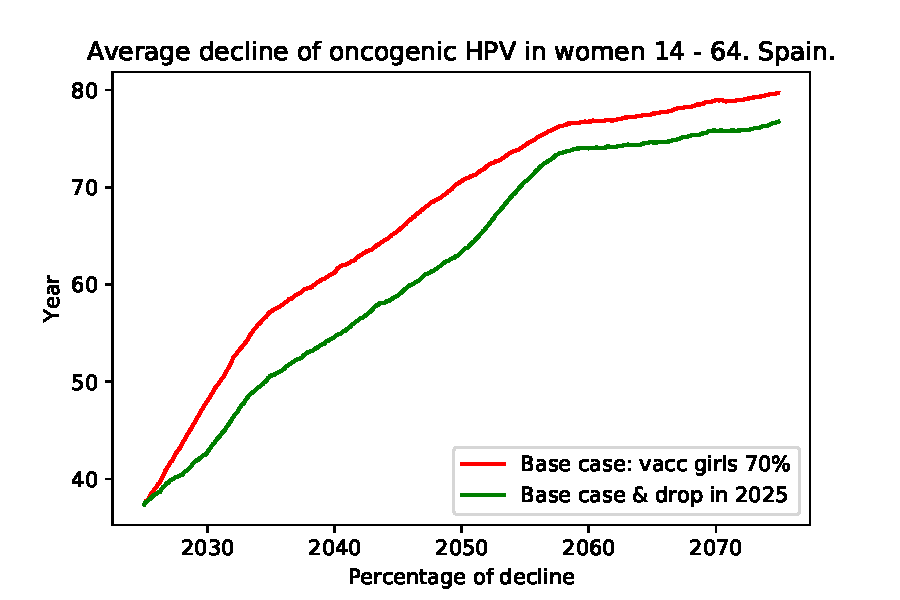
\includegraphics[width=0.5\linewidth]{IMGs/11.-Resilencia/Base_y_3/decline_onco_muj.pdf}	& 
		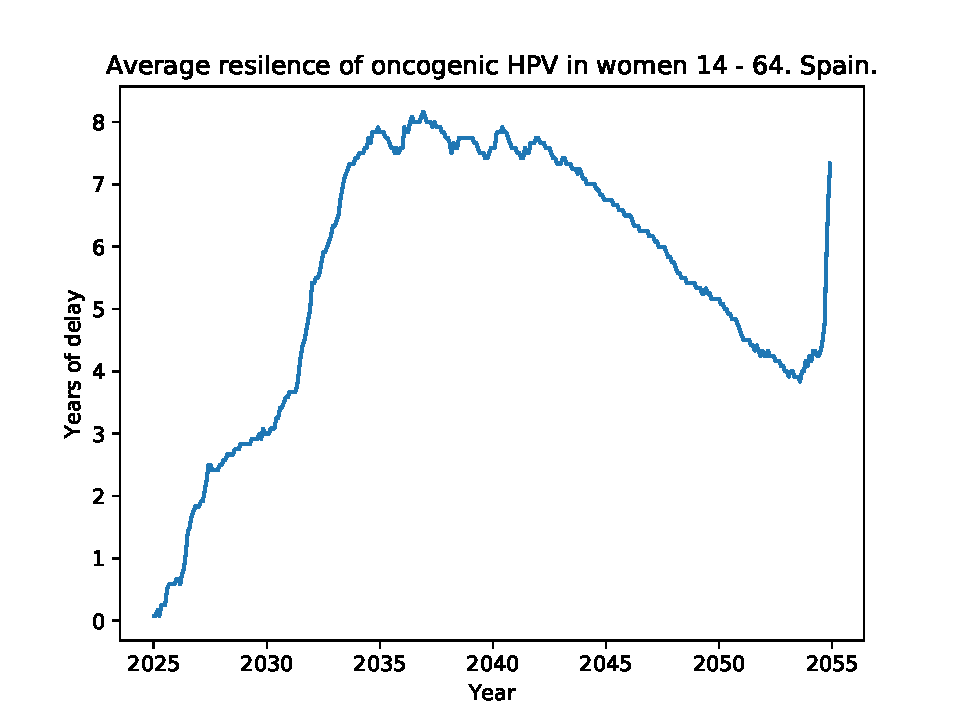
\includegraphics[width=0.5\linewidth]{IMGs/11.-Resilencia/Base_y_3/resilencia_onco_muj.pdf}  \\ 
		(c)	& (d) \\
	\end{tabular} 
	\caption{Comparative of Base Case and Case 3. On the left column, the average decline of oncogenic HPV in men (a) and women (c), in both cases. On the right column, the time (in years) the Case 3 needs to achieve the same levels of decline as the Base Case for oncogenic HPV in men (b) and women (d).}
	\label{fig:baseCase_Case3}
\end{figure}

\begin{figure}[!]
	\centering
	\begin{tabular}{cc}
		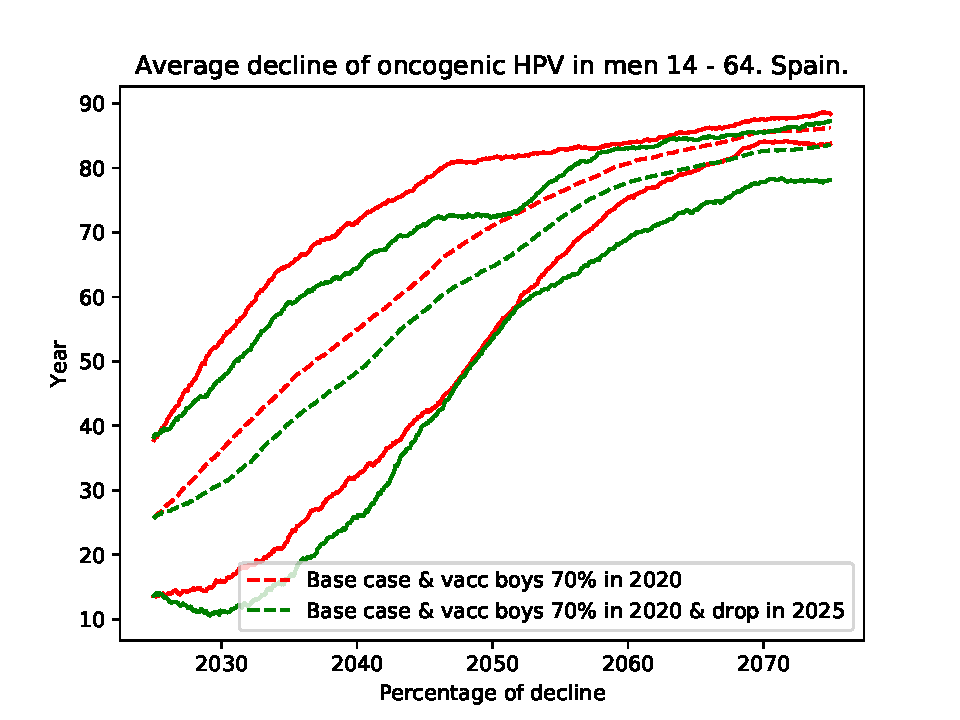
\includegraphics[width=0.5\linewidth]{IMGs/11.-Resilencia/2_y_4/decline_onco_hom.pdf}	& 
		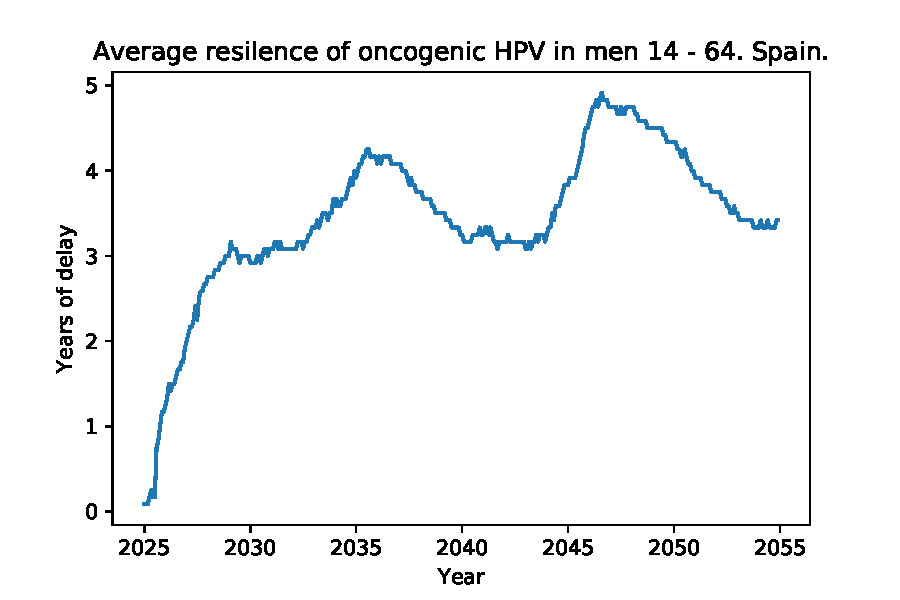
\includegraphics[width=0.5\linewidth]{IMGs/11.-Resilencia/2_y_4/resilencia_onco_hom.pdf}  \\ 
		(a)	& (b) \\ 
		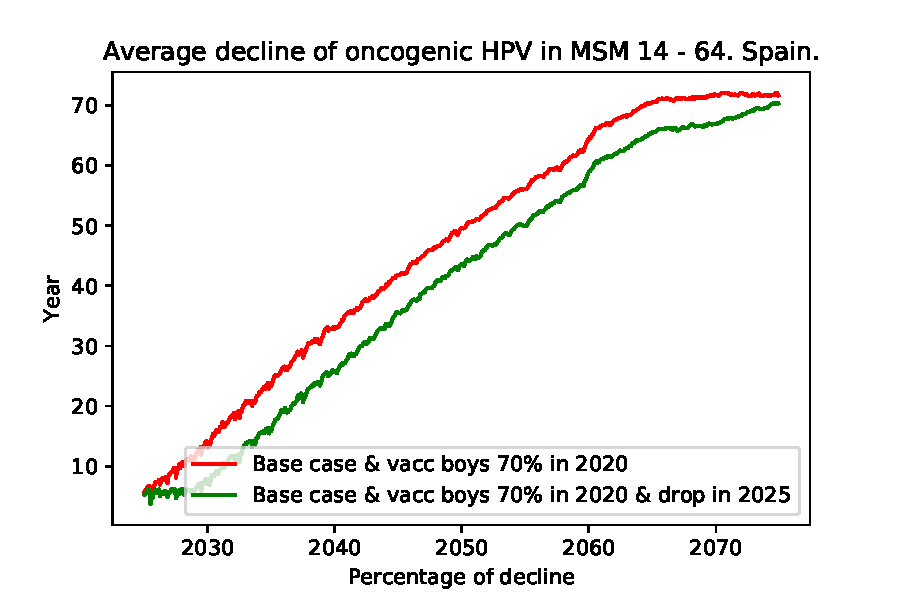
\includegraphics[width=0.5\linewidth]{IMGs/11.-Resilencia/2_y_4/decline_onco_MSM.pdf}	& 
		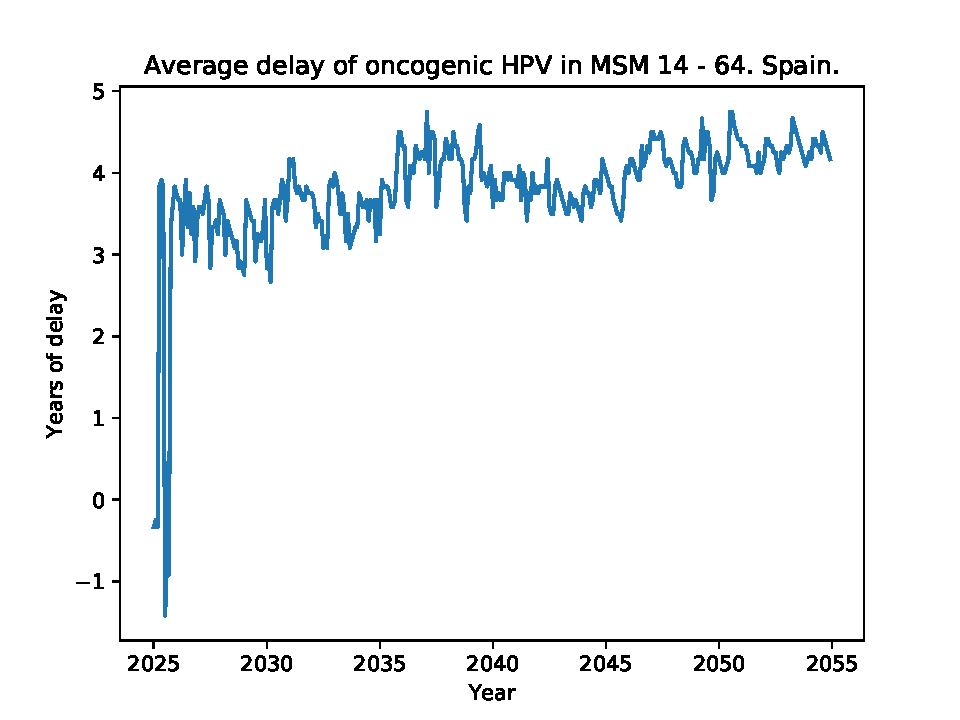
\includegraphics[width=0.5\linewidth]{IMGs/11.-Resilencia/2_y_4/resilencia_onco_MSM.pdf}  \\ 
		(c)	& (d) \\
		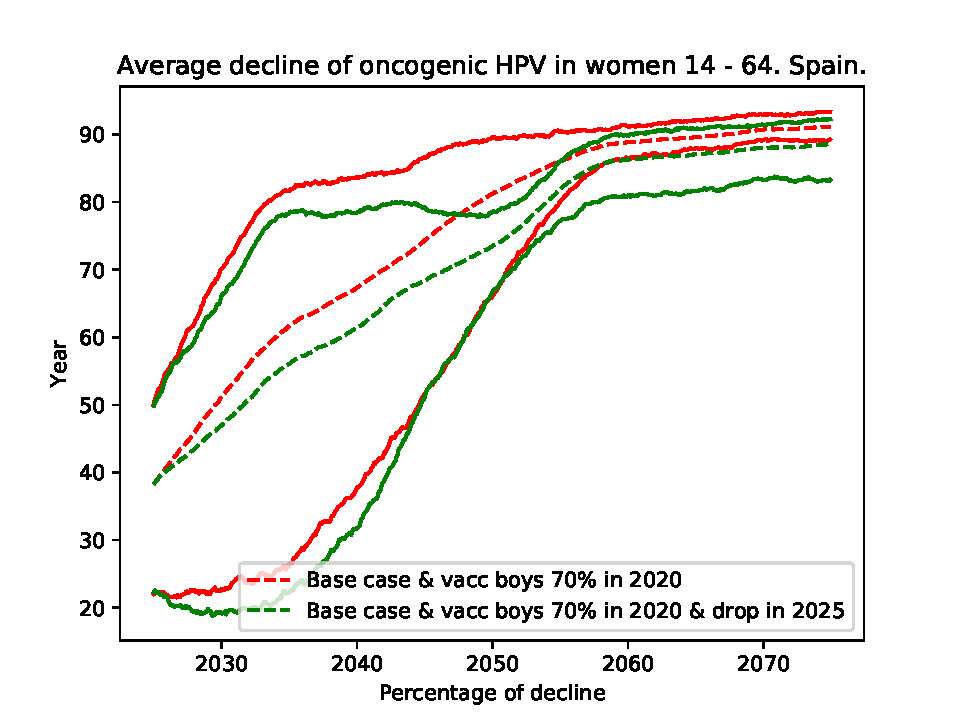
\includegraphics[width=0.5\linewidth]{IMGs/11.-Resilencia/2_y_4/decline_onco_muj.pdf}	& 
		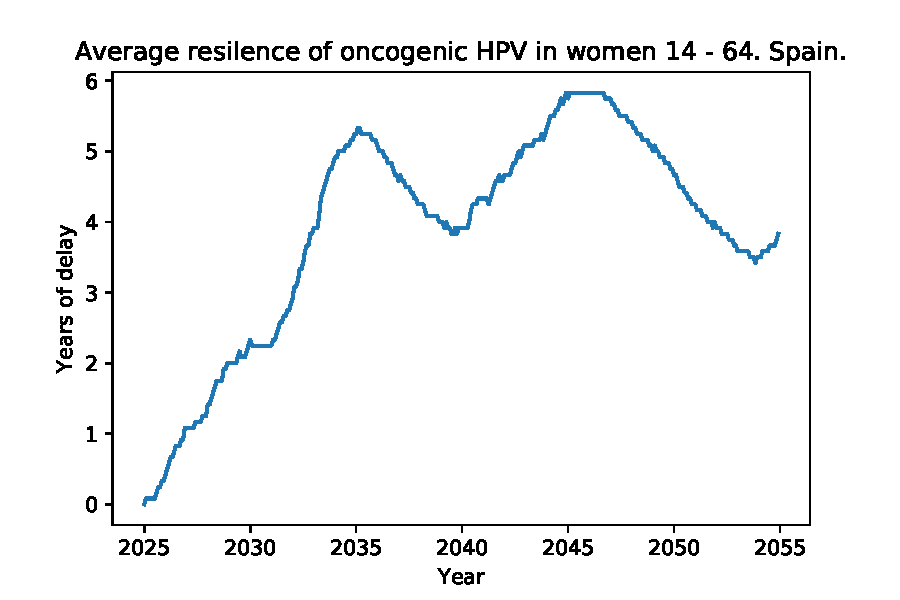
\includegraphics[width=0.5\linewidth]{IMGs/11.-Resilencia/2_y_4/resilencia_onco_muj.pdf}  \\ 
		(e)	& (f) \\  
	\end{tabular} 
	\caption{Comparative of Case 2 and Case 4. On the left column, the decline of oncogenic HPV in men (a), MSM (c) and women (e), in both cases. On the right column, the average time (in years) the Case 4 needs to achieve the same levels of decline as the Case 2 for oncogenic HPV in men (b), MSM (d) and women (f).}
	\label{fig:Case2_Case4}
\end{figure}

If we look at the left columns, the CI$95\%$ begin to converge from $2060$ for men and women, having a significant intersection. In MSM the parallelism is the same all the time.

Furthermore, when the decline starts to saturate, a short increase in the decline takes much longer time. Now, looking at the right columns:

\begin{itemize}
\item Men: in men, we can see that when boys and girls are vaccinated, the resilience is much less. We can see more clearly the differences in Figure \ref{fig:compara_resilencia}(a). In the maxima values, the difference is from $5\%$ to $12\%$.
\item MSM: it is interesting to notice that in \ref{fig:Case2_Case4}(d), the delay is practically constant over the time and equal to $4$ years. It may be because the small herd immunity effect on MSM.
\item Women: here, the difference is lower because in all the cases women are vaccinated. Nevertheless, there is an extra herd immunity effect when boys and girls are vaccinated that reduces in some years the delay.
\end{itemize}

In Figure \ref{fig:compara_resilencia} we plot in the same graphic, on the one hand,  \ref{fig:baseCase_Case3}(b) and \ref{fig:Case2_Case4}(b) to compare the resilience in men, and on the other hand, \ref{fig:baseCase_Case3}(f) and \ref{fig:Case2_Case4}(f) to compare the resilience in women. Here, the differences can be visualised more clearly.

\begin{figure}[!]
	\centering
	\begin{tabular}{cc}
		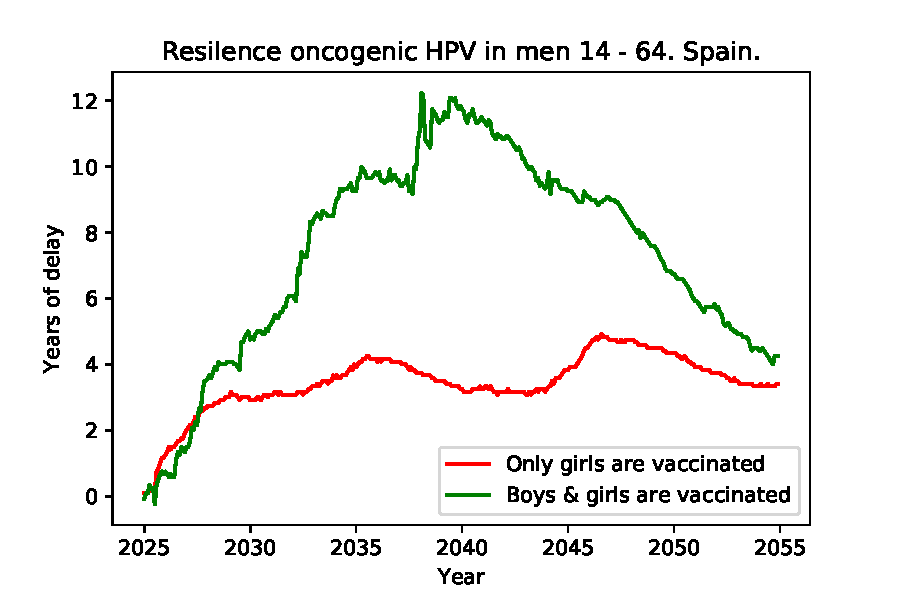
\includegraphics[width=0.5\linewidth]{IMGs/11.-Resilencia/compara_resilencia_onco_hom.pdf}	& 
		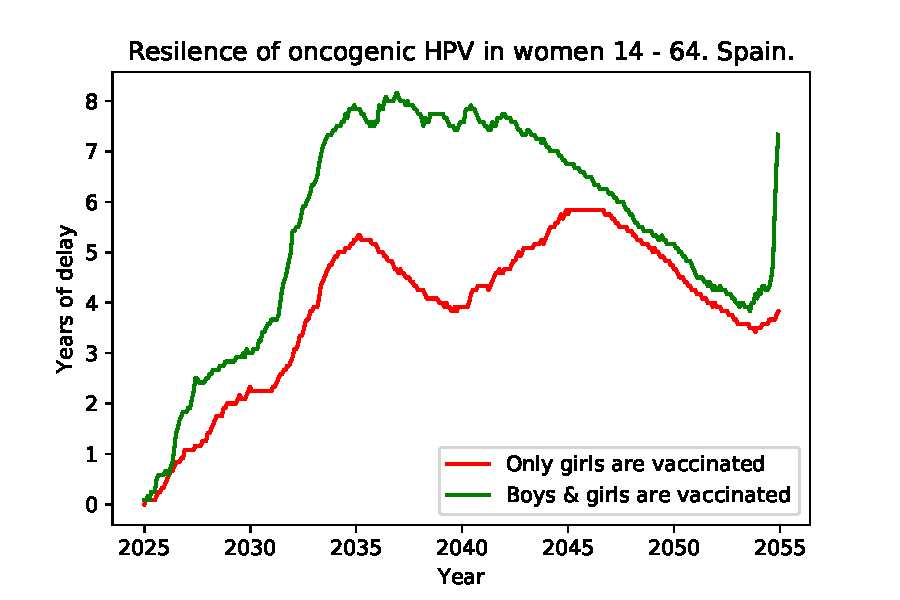
\includegraphics[width=0.5\linewidth]{IMGs/11.-Resilencia/compara_resilencia_onco_muj.pdf}  \\ 
		(a)	& (b) \\ 
	\end{tabular} 
	\caption{Comparative of the average time in years of the delay in the case where only girls are vaccinated and boys and girls are vaccinated. On the left (a), the average resilience of oncogenic HPV in men. On the right (b), the same as (a) but for women. The vaccination programs are more resilent when only girls are vaccinated.}
	\label{fig:compara_resilencia}
\end{figure}

Thus, we conclude that the vaccination programs are less resilent when boys and girls are vaccinated and, with the simulated programs, it is necessary $30--35$ years after the coverage has been recovered to see the convergence in the decline.
